\documentclass[12pt, preprint]{aastex}
\usepackage{graphicx}	% For figures
\usepackage{natbib}	% For citet and citep
\usepackage{amsmath}	% for \iint
\usepackage{bbm}	% for blackboard bold numbers
\usepackage[breaklinks]{hyperref}

\newcommand{\sex}{{\tt SExtractor}}

%\slugcomment{To be submitted}

\shorttitle{Probabilistic Stellar Catalogs}
\shortauthors{Brewer et al.}

\begin{document}

\title{Probabilistic Catalogs for Crowded Stellar Fields}

\author{Brendon J. Brewer\thanks{\texttt{bj.brewer@auckland.ac.nz}}}
\affil{Department of Statistics, The University of Auckland,
Private Bag 92019, Auckland 1142, New Zealand}

%\author{}

\author{Daniel Foreman-Mackey}
\affil{Center for Cosmology and Particle Physics, Department of Physics,
New York University, Washington Place, New York, NY, 10003, USA}

\and

\author{David W. Hogg}
\affil{Center for Cosmology and Particle Physics, Department of Physics,
New York University, Washington Place, New York, NY, 10003, USA}

\begin{abstract}
We introduce a probabilistic (Bayesian) method for producing catalogs
from images of crowded stellar fields. The method is capable of inferring the
number of sources $N$ in the image and can also handle the
challenges introduced by overlapping sources. The luminosity
function of the stars can also be inferred even when the precise luminosity of each star is uncertain.
This is in contrast with standard techniques which produce a single catalog,
potentially underestimating the uncertainties in any study of the stellar
population and discarding information about sources at or below the detection limit. The method is implemented using advanced Markov Chain Monte Carlo
(MCMC) techniques including Reversible Jump and Nested Sampling.
The computational feasibility of the method is
demonstrated on simulated data where the luminosity function of the stars is a
broken power-law. The parameters of the luminosity function can be recovered
with moderate uncertainties. We compare the results obtained from our method
with those obtained from the \sex~software and find that the latter significantly
underestimates the number of stars in the image and leads to incorrect
inferences about the luminosity function of the stars.
\end{abstract}

\keywords{catalogs --- methods: data analysis --- methods: statistical ---
stars: luminosity function, mass function}

\section{Introduction}
Traditional practice in astronomy is to take images of the sky, detect
or enumerate sources visible in those images, and create catalogs.
These catalogs are then used to perform the fundamental astronomical
measurements, which might include something like the three-dimensional
structure of the Galaxy or the two-point correlation function of
galaxies.  Indeed, the process of catalog construction is so ``baked
in'' to our ideas about what astronomy is, we sometimes forget that
the catalog is \emph{not} the fundamental data product of astronomy; catalogs are produced
from imaging; their production involves many decisions and ideas
that go way beyond the information provided to the telescope by the
incident intensity field. In addition, catalogs are not usually the final
goal of any imaging project or survey. Typically, they are produced in
order to facilitate the scientific study of populations of objects (e.g. the
initial mass function of a population of stars), or to provide a sky-search
capability to the community who might be interested in only a small subset of
objects. Standard tools for generating catalogs from astronomical imaging
include \sex~\citep{sextractor}, DAOPHOT \citep{1987PASP...99..191S}, and SDSS
PHOTO \citep{photo}.

Telescopes don't make catalogs \citep{2011EAS....45..351H}, they
measure the intensity field.  Viewed through the lens of probabilistic
inference, the goals of astronomy are to take the information in the
telescope-generated records of the intensity field and deliver it to
the quantities of astronomical interest with as little loss as
possible.  Insertion of a catalog-generation step in the inference
pipeline between the raw imaging and the final astrophysical analyses
is typically very lossy; the hard decisions of catalog making destroy
information.  Probability theory suggests that it will be much less
lossy to pass forward not a catalog but a probabilisitic
description of all the catalogs that could be consistent with the
imaging---a posterior probability in (enormously large) catalog space.
This article represents an attempt at this ambitous goal in the specific
situation where the only objects in the field are stars.

Beyond these extremely general concerns, there are practical issues:
Standard methods for constructing catalogs can have difficulty in some
challenging situations. For example, when multiple sources overlap partially
or completely, it can be difficult to determine how many sources are present,
and how much flux belongs to each source. In principle, uncertainty should be
taken into account. Instead of simply {\it estimating} the position and flux of
each object in the image, we should fully describe the fact that sometimes we
are not certain of the position and flux of each source. This uncertainty
should then be propagated into any inferences about the stellar population.

Essentially, the creation of a catalog is an attempt to answer the question,
``Given the image we have obtained, what objects are present in the field and
what are their properties?'' This motivates a probabilistic (Bayesian)
approach to making catalogs. The output of such an approach would not be a
single answer to this question (i.e. a single ``point estimate'' catalog), but
rather a posterior probability distribution over the space of possible catalogs.
Numerically, Bayesian Inference is often implemented using Markov Chain Monte
Carlo (MCMC) algorithms in order to generate random samples from the posterior
distribution.

Sampling a posterior probability distribution for catalogs is likely to be
challenging for a number of reasons. Firstly, the number $N$ of objects in the
image (and that should therefore be listed in the catalog) is itself unknown.
Secondly, if $N$ is large, then the parameter space
of positions and properties (flux, size, etc) of the objects is also large.
This can cause Markov Chain Monte Carlo (MCMC) algorithms difficulties -- they
may take a long time to converge to the target posterior distribution over
the space of catalogs. Thirdly, this problem is subject to the so-called
label-switching problem that is commonly encountered in mixture modeling
\citep[e.g.][]{label_switching}. Given any proposed catalog, another catalog that is
equally plausible is the catalog obtained by shuffling the entries of the first
catalog. This leads to a posterior distribution with $N!$ identical peaks in
parameter space. This can lead to difficulties with certain (generally very
effective) MCMC algorithms such as the affine-invariant stretch move
\citep{goodman, emcee}.

Bayesian object detection (as this problem is sometimes called) has been
implemented both inside and outside of astronomy
\citep[e.g.][]{object, 2003MNRAS.338..765H, 2011MNRAS.415.3462F}. However, the
\citet{2011MNRAS.415.3462F} approach makes the assumption of a
known number of objects $N$.
This assumption is required for the
{\tt MultiNest} sampler \citep{multinest} to be applicable.
Using the results from the known $N$
run, it is possible (under certain circumstances) to reconstruct what the
results would have been if an unknown-$N$ model had been used. However,
this will not work well in situations where there is significant confusion
(i.e. two or more sources overlap). What is really required is a variable
dimension model, where $N \in \{0, 1, 2, ... \}$ is an unknown quantity to be
inferred from the data.
The computational implementation of these models will require tools such as
reversible jump Markov Chain Monte Carlo \citep{rjmcmc}. Other statistical
methods have also been used to model crowded fields
\citep[e.g. maximum likelihood,][]{irwin}.
However, maximum likelihood is not completely appropriate in flexible models
because it may lead to overfitting. In this situation overfitting would result
in more stars being added to the model to explain small positive fluctuations
in the image which are actually due to noise. Various other techniques have
also been proposed in the literature \citep[e.g.][]{2002MNRAS.335...73M, 2007A&A...461..373M, 2009PASP..121.1429Z}.

\section{Bayesian Inference}
To quantitatively model uncertainties and transform noise in observed data
into uncertainties in parameters of interest, Bayesian Inference is the appropriate
framework \citep{cox, jaynes, caticha, mackay}. Suppose there exist unknown parameters
(denoted
collectively by $\theta$) and we expect to obtain some data $x$. Our prior
state of knowledge about the parameters is modelled by a prior
probability distribution:
\begin{equation}
p(\theta).
\end{equation}
Note that this is a very concise notation \citep{hogg} and should be read
as ``the probability distribution for $\theta$''.
We also model how the parameters give rise to the data, via a generative model.
This is also known as a {\it sampling distribution}:
\begin{equation}
p(x|\theta).
\end{equation}
Despite the singular, the sampling distribution is actually a family of
probability distributions over the space of possible data sets, one probability
distribution for each possible value
of $\theta$. Note that the choice of
the sampling distribution is also an assumption about prior knowledge:
It models prior information about the fact that the data $x$ is connected to
the parameters $\theta$ in some way. Without this prior knowledge, learning is
impossible: there has to be some relationship between the parameters and the
data, otherwise new data tells you about nothing but itself.

When specific data $x^*$ have been obtained, our state of knowledge about $\theta$
gets updated from the prior distribution to the posterior distribution
via Bayes' rule:
\begin{eqnarray}
p(\theta|x=x^*) &\propto& p(\theta)p(x|\theta)|_{x=x^*} \\
&=& p(\theta)\mathcal{L}(\theta; x)
\end{eqnarray}
The term $p(x|\theta)|_{x=x^*} = \mathcal{L}(\theta; x)$
is the {\it likelihood function}, which is the
probability of obtaining the actual data set $x^*$ as a function of the
parameters. In the case that the sampling distribution is a probability
density, the likelihood is the probability density function evaluated at the observed
data. This usually causes no problems, although one should be aware of the
Borel-Kolmogorov paradox \citep{jaynes}.
As suggested by the above notation, the likelihood function is obtained from the
sampling distribution with the actual data substituted in and is therefore
a function of the parameters only.

To proceed with the model for inferring catalogs (stellar positions and fluxes)
from image data, we must
specify a definite hypothesis space and choices for the prior distribution
and the sampling distribution. These choices are presented and discussed in
Section~\ref{sec:model}. In Section~\ref{sec:mcmc} we briefly discuss our
MCMC implementation. Section~\ref{sec:simulated_data} describes the tests we
carried out on simulated data, and a comparison with \sex~results is presented
in Section~\ref{sec:sex}. We conclude in Section~\ref{sec:conclusion}.
%Throughout this paper we make a number of simplifications
%for the purposes of testing the computational feasibility and performance of
%the method. In real applications, some of these assumptions (such as known PSF
%and noise variance) may be relaxed.

\section{The Specific Model for Stellar Fields}\label{sec:model}
\subsection{The Hypothesis Space}
The hypothesis space is the set of possible catalogs, or the set of possible
answers to the question, ``What objects are present in the field and
what are their properties?'' We shall assume that there are an unknown number of stars
$N$ in the field. Each star has an unknown
position $(x,y)$ in the plane of the sky, and an unknown flux $f$. We also
describe the distribution of fluxes (commonly known as the {\it luminosity
function}) of the stars by some parameters denoted collectively by $\beta$.
In summary, the unknown parameters are:
\begin{eqnarray}
\theta = \left\{N, \beta, \left\{x_i, y_i\right\}_{i=1}^N,
\left\{f_i\right\}_{i=1}^N\right\}.
\end{eqnarray}
We note that models similar to this have been implemented for general image
modeling and deconvolution \citep[e.g.][]{massinf}, however in this case it is
more justified as we are actually searching for point fluxes.

\subsection{The Prior}
The prior probability distribution for the unknown parameters can be factorized
using the product rule of probability theory.
With a variety of independence assumptions, the prior
can be factorized as:
\begin{eqnarray}
p(\theta) = p(\beta)p(N|\beta)\prod_{i=1}^N p(x_i, y_i)
p(f_i | \beta)
\end{eqnarray}
Here, we have assumed that the luminosity function does not depend on position.
Finally, the fluxes of the stars come independently from
a common distribution. If we knew the luminosity
function of the stars, then the location and flux of a particular star would
not tell us anything about the location and flux of another star. Really, this
is just a way of implementing exchangeability of the stars.

For simplicity, we assume a uniform prior probability distribution for the
position of each star. This creates a strong preference for catalogs where
the stars are uniformly distributed across the image. Thus, this model is
appropriate for small patches of sky where the density of stars is approximately
uniform. In other scenarios, such as images of stellar clusters, it is possible
to parameterize the spatial distribution of the stars in a similar way to how
we have parameterized the luminosity function.

\subsection{The Sampling Distribution}
The sampling distribution is a probabilistic model for the process that
generates the data; it describes the probability distribution we would use
to predict the data if we happened to know the true catalog. In our case,
the data will be an $m \times n$ array of pixel intensities $I$:
\begin{eqnarray}
\{I_{ij}\}
\end{eqnarray}
where the central position of each pixel is:
\begin{eqnarray}
\{X_{ij}, Y_{ij}\}.
\end{eqnarray}
The image is assumed to be a noisy version of the true underlying intensity
field. Thus, we need
a prescription for simulating an image $\{I_{ij}\}$ from a catalog $\theta$:
\begin{eqnarray}
\theta = \left\{N, \beta, \left\{x_i, y_i\right\}_{i=1}^N,
\left\{f_i\right\}_{i=1}^N\right\}.
\end{eqnarray}
If we knew the true catalog, we could compute the
``mock image'' we would expect to see
in the absence of noise. This mock image (defined at every point on the sky)
is given by:
\begin{eqnarray}
\mathcal{M}(x, y) &=& \sum_{i=1}^N f_i \mathcal{P}(x - x_i, y - y_i)
\end{eqnarray}
where $\mathcal{P}$ is the pixel-convolved point spread function (PSF).
Throughout this paper we will
assume the pixel-convolved PSF is a weighted mixture of two concentric
circular
Gaussians with widths $s_1$ and $s_2$:
\begin{eqnarray}
\mathcal{P}(x, y) = \frac{w}{2\pi s_1^2}\exp
\left[
-\frac{1}{2s_1^2}\left(x^2 + y^2\right)
\right]
+ \frac{1-w}{2\pi s_2^2}\exp
\left[-\frac{1}{2s_2^2}\left(x^2 + y^2\right)
\right].
\end{eqnarray}
The pixellated observed image is assumed to be generated from the mock
image (evaluated at the center of each pixel) plus noise:
\begin{eqnarray}
I_{ij} &=& \mathcal{M}(X_{ij}, Y_{ij}) + \epsilon_{ij}
\end{eqnarray}
where the errors $\{\epsilon_{ij}\}$ are independent and normally distributed.
The variance of each pixel is determined by the brightness of the sky and the
brightness of the mock image in that pixel:
\begin{eqnarray}
\epsilon_{ij} \sim \mathcal{N}(0, \sigma_0^2 + \eta \mathcal{M}(X_{ij}, Y_{ij})).
\end{eqnarray}
where $\sigma_0$ is a constant noise level and $\eta$ is a coefficient allowing
the noise to be higher in brighter regions of the image.
This parameterisation has been used by \citet{2011MNRAS.412.2521B} and is an
alternative to the common practice of producing a ``variance map'' from the
image data that is then assumed to be known.

\subsection{The Prior Distribution}
The prior distribution for the number of stars $N$ is assigned to be uniform
between 0 and some maximum number $N_{\rm max}$. The extent of the image is
assumed to be from $x=x_{\rm min}$ to $x=x_{\rm max}=x_{\rm min} + x_{\rm range}$ and from
$y=y_{\rm min}$ to $y=y_{\rm max}=y_{\rm min} + y_{\rm range}$ in arbitrary units, and the
positions of the stars are assigned independent uniform priors:
\begin{eqnarray}
x_i &\sim& \textnormal{Uniform}(x_{\rm min} - 0.1x_{\rm range}, x_{\rm max} + 0.1x_{\rm range}) \\
y_i &\sim& \textnormal{Uniform}(y_{\rm min} - 0.1y_{\rm range}, y_{\rm max} + 0.1y_{\rm range})
\end{eqnarray}
The stars are allowed to be slightly outside of the observed image because the
PSF can scatter light from these stars into the image. Our model for the
luminosity function is a broken power-law with four
free parameters:
\begin{eqnarray}
\beta = \{h_1, h_2, \alpha_1, \alpha_2\}.
\end{eqnarray}
where $h_1$ is a lower flux limit, $h_2$ is a break-point, $\alpha_1$ is
the slope of the distribution between $h_1$ and $h_2$, and $\alpha_2$ is the
slope of the distribution above $h_2$. For details on the broken power-law
model, see Appendix~\ref{power_law}. The prior distribution on $h_1$, $h_2$,
$\alpha_1$, and $\alpha_2$ is assigned to be:
\begin{eqnarray}
\ln h_1 &\sim& \textnormal{Uniform}(\ln(10^{-3}), \ln(10^3)) \\
\ln h_2 &\sim& \textnormal{Uniform}(\ln(h_1), \ln(h_1) + 2.3) \\
\alpha_1 &\sim& \textnormal{Uniform}(1, 5) \\
\alpha_2 &\sim& \textnormal{Uniform}(1, 5).
\end{eqnarray}
These priors express vague prior knowledge about $\alpha_1$ and $\alpha_2$ in
addition to vague prior knowledge about $h_1$ and $h_2$ apart from the fact
that the flux units are not extreme and that $h_2$ should be no more than an
order of magnitude greater than $h_1$.

This simply-parameterized model for the luminosity function can be criticized
on the basis that information from bright stars can be used to infer the
parameters of the luminosity function which then still apply at lower flux
levels. In principle, this can be resolved by using a more flexible distribution
\citep[e.g.][]{2008ApJ...682..874K} where each star's measured brightness
affects the inference of the luminosity function locally but not globally.

The priors for the PSF parameters and the noise parameters were:
\begin{eqnarray}
\ln s_1 &\sim& \textnormal{Uniform}(\ln(0.3L), \ln(30L)) \\
\ln s_2 &\sim& \textnormal{Uniform}(\ln(s_1), \ln(s_1) + 2.3) \\
w &\sim& \textnormal{Uniform}(0, 1)\\
\ln \sigma_0 &\sim& \textnormal{Uniform}(\ln(10^{-3}), \ln(10^{3})) \\
\ln \eta &\sim& \textnormal{Uniform}(\ln(10^{-3}), \ln(10^{3}))
\end{eqnarray}
where $L = (x_{\rm max} - x_{\rm min})/n$ is the width of a pixel.

\section{MCMC Implementation}\label{sec:mcmc}
The MCMC sampling was implemented using the Diffusive Nested Sampling
\citep{dnest} method (hereafter DNS). DNS is a variant of the
Nested Sampling \citep{skilling} algorithm that uses Metropolis-Hastings
updates, and
is very generally applicable. The main difference between DNS and the standard
Metropolis-Hastings algorithm is that the target distribution is modified.
Rather than simply exploring the posterior distribution over catalog space,
DNS constructs an alternative target distribution which is a mixture of the
prior distribution with more constrained versions of the prior distribution.
The modified target distribution assists the sampling in several ways.
Firstly, the target distribution shrinks at a constant rate with time during the
initial phase of the exploration. This is similar to the popular ``simulated
annealing'' method \citep{annealing, neal} but with an optimal annealing schedule. Secondly,
communication with the prior is maintained: once a catalog is found that
fits the data, the catalog can ``disintegrate'' back to the prior distribution
and re-fit, allowing different peaks in the parameter space to be explored
(if they exist). This all happens naturally within the context of a valid
MCMC sampler. The MCMC may also be run using the standard Metropolis algorithm
targeting the posterior distribution.

\section{Simulated Data}\label{sec:simulated_data}
In order to test our approach, we applied the method to two illustrative
simulated images generated from
the above model. The purpose of this experiment was to test the computational
feasibility of the model, as well as to compare the inferences from the model
with those from more standard techniques.

The true parameter values for the two simulated data sets are listed in
Table~\ref{tab:truth}. The broken power-law parameter values were chosen so that
roughly half of the stars' fluxes were below and above the break-point
respectively. Figure~\ref{fig:powerlaw} in Appendix~\ref{power_law} also shows the true flux distribution
used for the simulated images. Each of the images
is $100 \times 100$ pixels in extent and covers a range from $-1$ to $1$ in
arbitrary units for both the $x$ and $y$ axes. The first image contains
100 stars (including stars just outside of the image; there are 63 stars actually
centered within the image) and the second
image contains $\sim$1000 stars (699 of which are centered within the image).
The two simulated images themselves
are shown in Figure~\ref{fig:simulated_data}.

\begin{table}\footnotesize
\begin{center}
\begin{tabular}{|c|c|c|}
\hline
Parameter & Value (Test Case 1) & Value (Test Case 2)\\
\hline
$N$ & 100 & 1000\\
$h_1$ & 0.3 & 0.3\\
$h_2$ & 0.6 & 0.6\\
$\alpha_1$ & 1.1 & 1.1\\
$\alpha_2$ & 2 & 2\\
\hline
$\sigma_0$ & 10 & 10\\
$\eta$ & 10 & 10 \\
$s_1$ & 0.02 & 0.02\\
$s_2$ & 0.1 & 0.1\\
$w$ & 0.5 & 0.5\\
\hline
\end{tabular}
\end{center}
\caption{True parameter values used to generate the simulated data. The main
difference between the two test cases is the number of stars and the noise
level, both of which are higher in test case 2.
\label{tab:truth}}
\end{table}

\begin{figure}[ht!]
\begin{center}
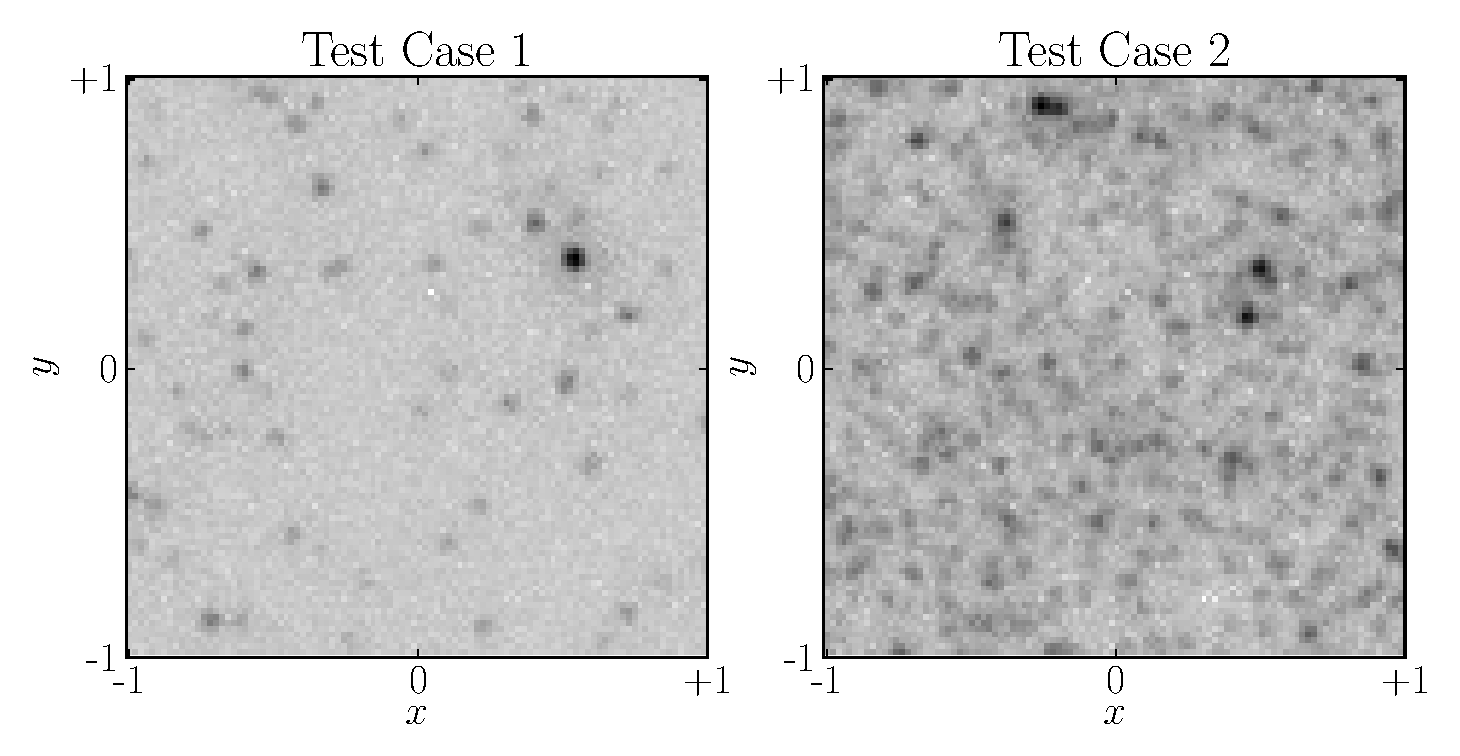
\includegraphics[width=\textwidth]{Figures/test_cases.eps}
\caption{The two simulated images used to test our methodology.
{\bf Left}: A field containing $\sim$100 stars.
{\bf Right}: A field containing $\sim$1000 stars.\label{fig:simulated_data}}
\end{center}
\end{figure}

\subsection{Test Case 1}
Test Case 1 was run with the DNS algorithm and usable results were obtained
within about an hour on a modern desktop PC. The inferences on the parameters
$N$, $h_1$, $h_2$, $\alpha_1$, and $\alpha_2$ are shown in
Figure~\ref{fig:results1}. The number of stars is correctly inferred, and the
posterior distributions for the other parameters comfortably contain the true
input values. Note that the uncertainty in $h_2$, $\alpha_1$, and $\alpha_2$ is
quite large. This is because the broken power-law model
(Figure~\ref{fig:powerlaw}) does not change drastically in shape as the
parameters are varied. Therefore, a large number of stars would be required to
tightly constrain the parameters. A Nested Sampling approach assists on
this problem because of the presence of a first-order phase transition
\citep{skilling}.

\begin{figure}[ht!]
\begin{center}
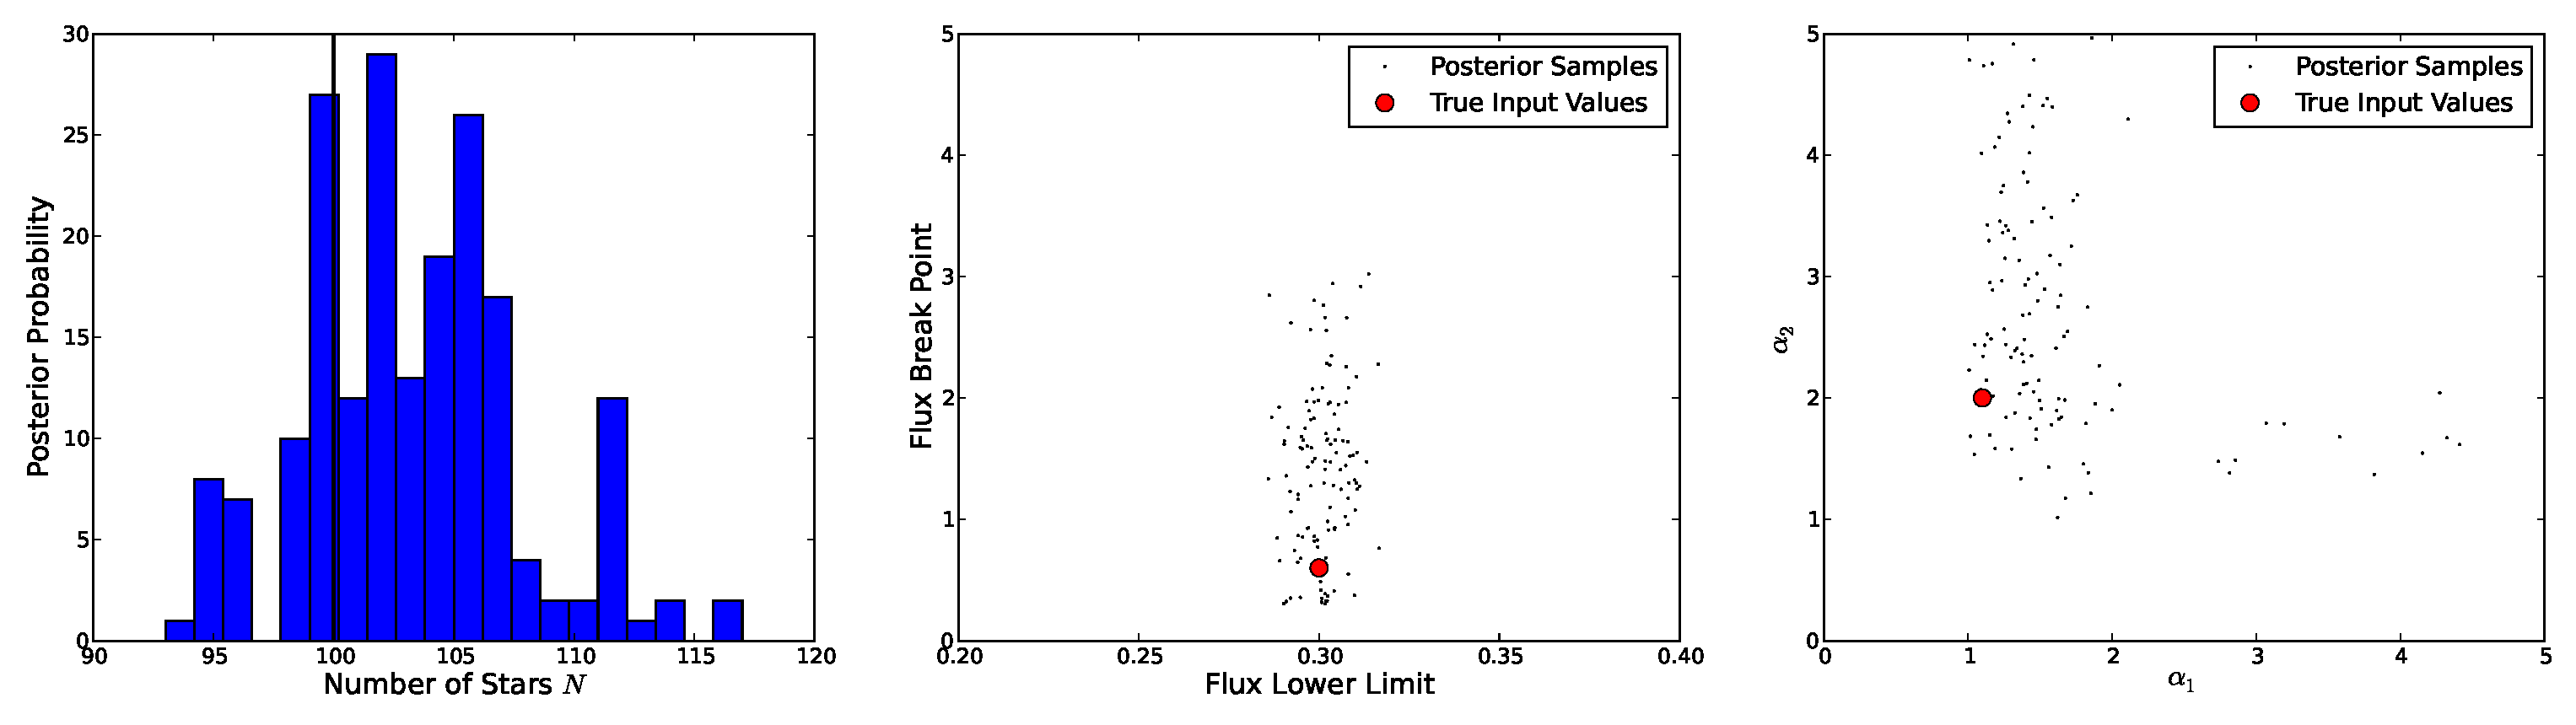
\includegraphics[width=\textwidth]{Figures/inference1.eps}
\end{center}
\caption{Inference about the parameters for Test Case 1. Note that there is
considerable uncertainty (particularly about $h_2$), which occurs because the
shape of the broken power-law does not depend strongly on the parameters.
The true input values are plotted as filled squares.
\label{fig:results1}}
\end{figure}

The PSF parameters $\{s_1, s_2, w\}$ and the noise parameters $\{\sigma_0, \eta\}$
were also inferred accurately with small uncertainties.

\subsection{Test Case 2}
Test Case 2 is more challenging than Test Case 1 because the image contains
more stars. This increases the size of the computational task in a number of
ways: firstly, there will be more unknown parameters to infer, so the
convergence of the MCMC algorithm will take longer. Secondly, the time taken
to compute the predicted image from a catalog (in order to evaluate the
likelihood) is longer because of the larger number of stars. Using DNS, some
samples from the posterior distribution can be obtained in about a day on a
modern PC. However, this problem does not have a first-order phase transition
like Test Case 1. Therefore, it is tractable to run standard Metropolis-Hastings
MCMC targeting the posterior distribution. In fact, this can be more efficient
because the degree of compression from the prior distribution to the posterior
distribution is very large ($\sim e^{3000}$) in this case.

\begin{figure}[ht!]
\begin{center}
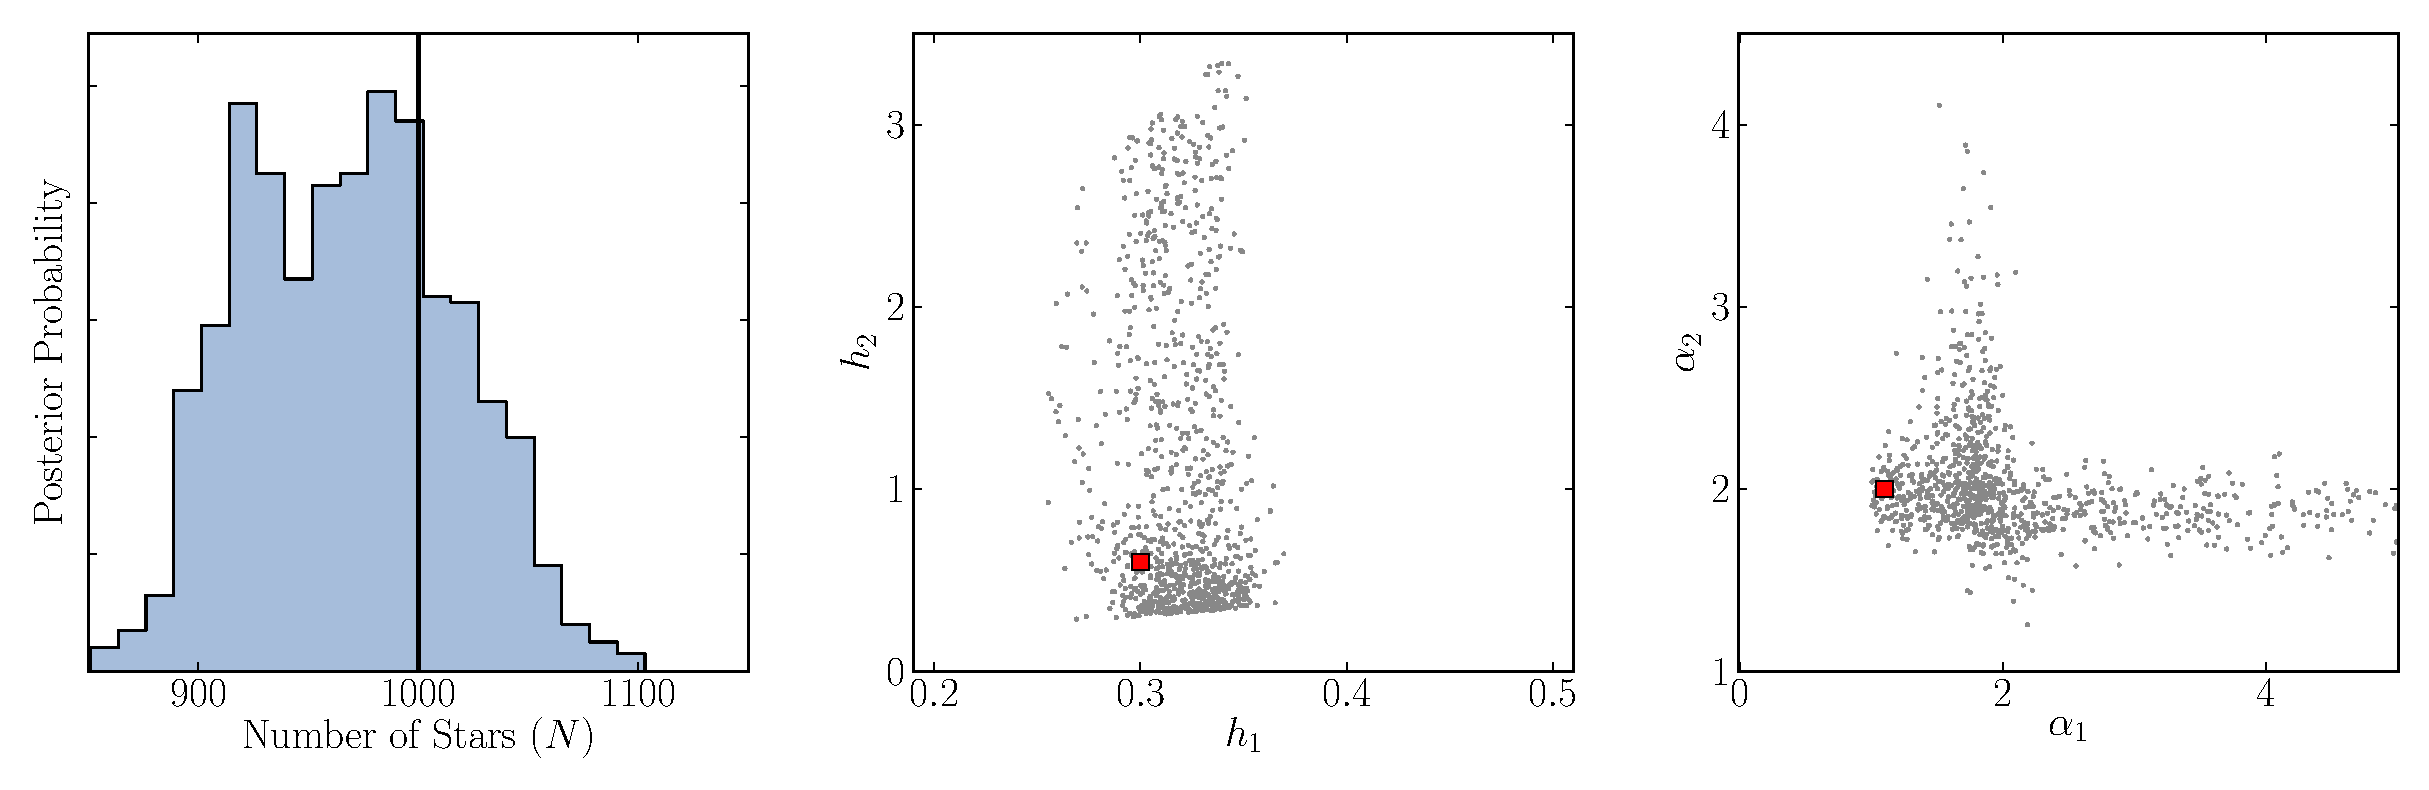
\includegraphics[width=\textwidth]{Figures/inference2.eps}
\end{center}
\caption{Inference about the parameters for Test Case 2. Note that the
parameters are still not very well constrained even with the larger number of
stars. The true input values are plotted as filled squares.\label{fig:results2}}
\end{figure}

Some summary results from Test Case 2 are shown in Figures~\ref{fig:catalogs}
and~\ref{fig:summaries}. Figure~\ref{fig:catalogs} shows nine possible catalogs
sampled from the posterior
distribution. Features that are common to these nine samples are plausible, and
features that differ are uncertain.

\begin{figure}[ht!]
\begin{center}
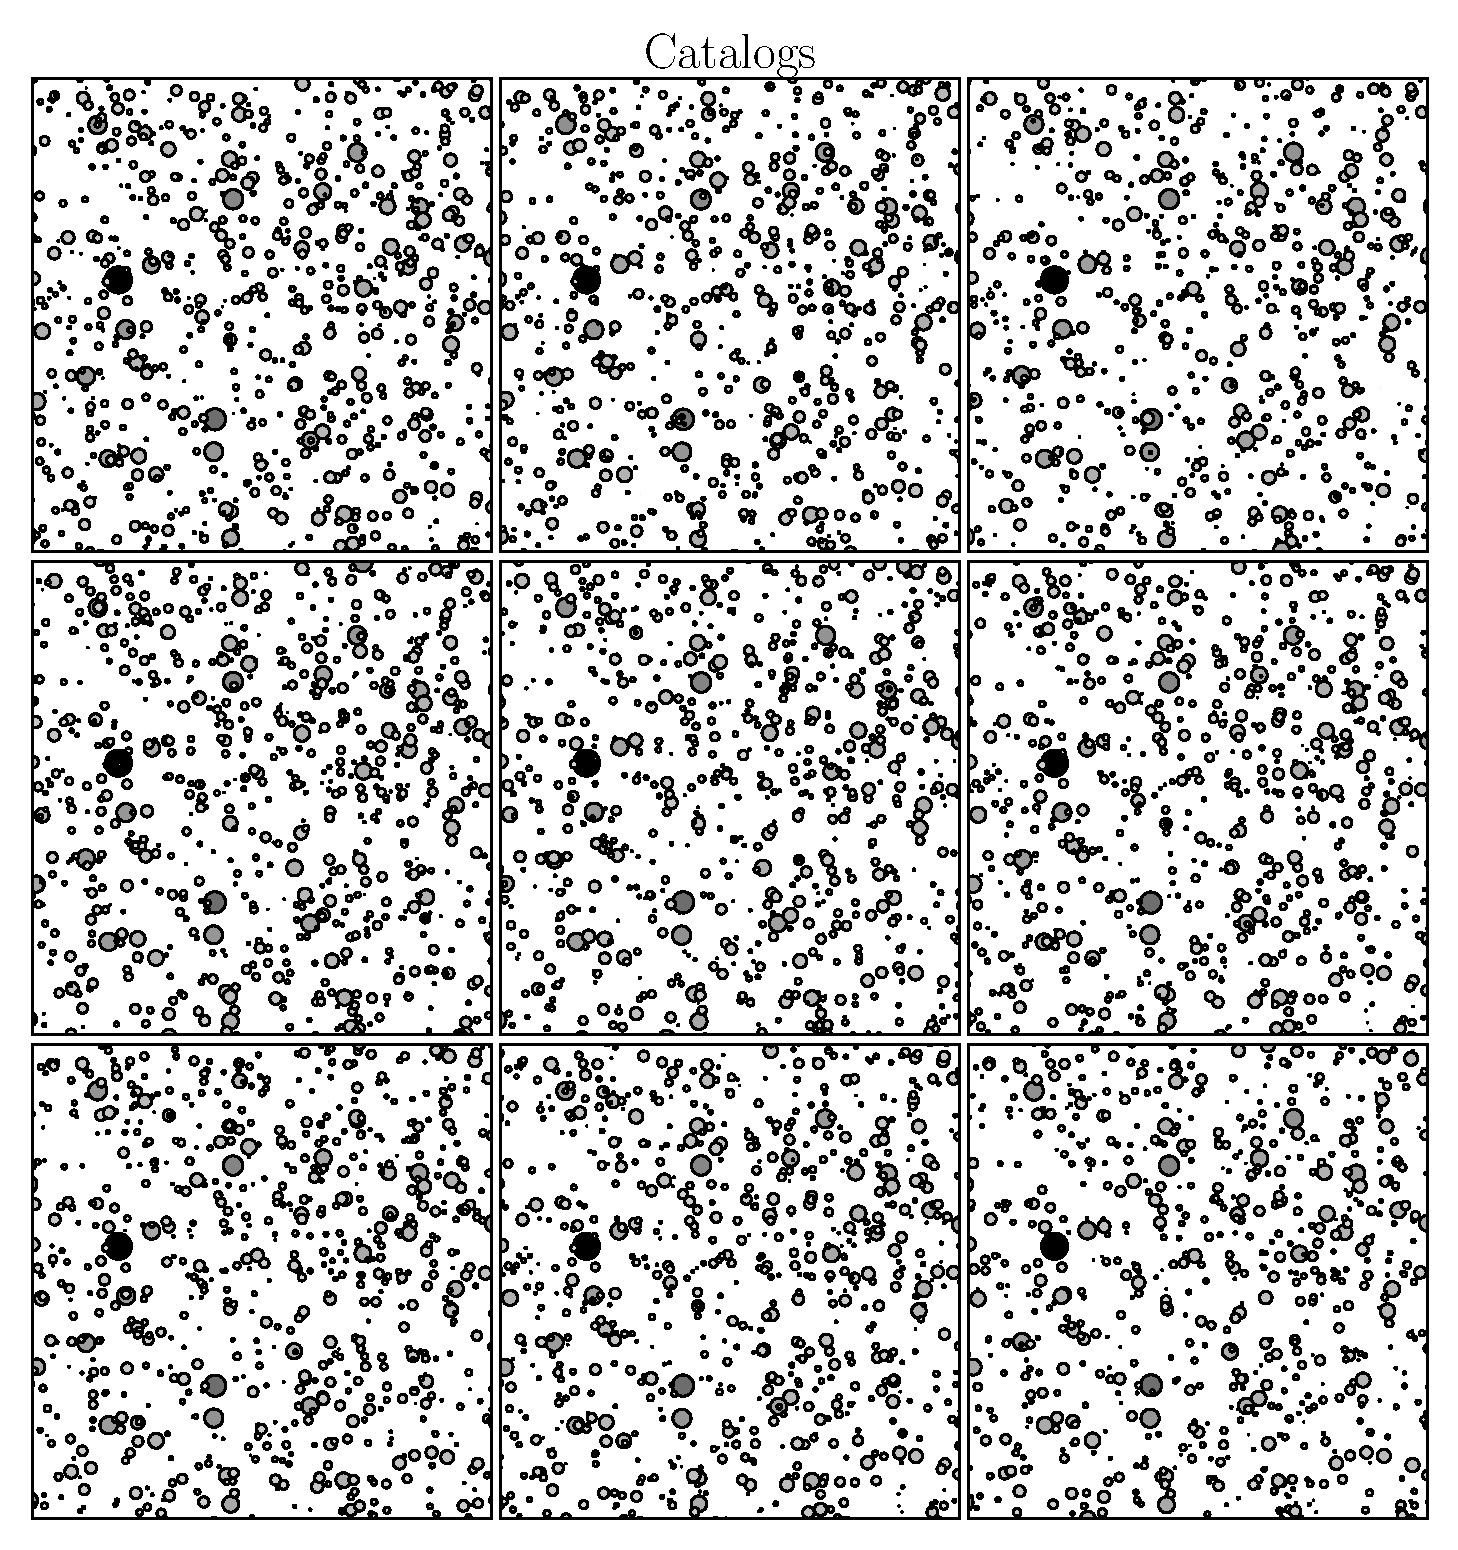
\includegraphics[scale=0.6]{Figures/catalogs.eps}
\end{center}
\caption{Nine example catalogs sampled from the posterior distribution for
Test Case 2. Features in common represent features with high probability,
and differences between the catalogs represent conclusions that are uncertain.
The area of each circle is proportional to the flux of the star.\label{fig:catalogs}}
\end{figure}

Each catalog in the posterior sample represents a scenario for the true
underlying image that we would observe if we had a hypothetical noise-free,
infinite resolution telescope. From these samples, we can construct the
posterior expected true scene. This is shown in Figure~\ref{fig:summaries} along
with the blurred (but still noise-free) version and the residuals. The residuals
provide a check on the validity of the model, and the posterior expected true
scene provides a useful visual guide to the uncertainties present in the catalogs.

\begin{figure}[ht!]
\begin{center}
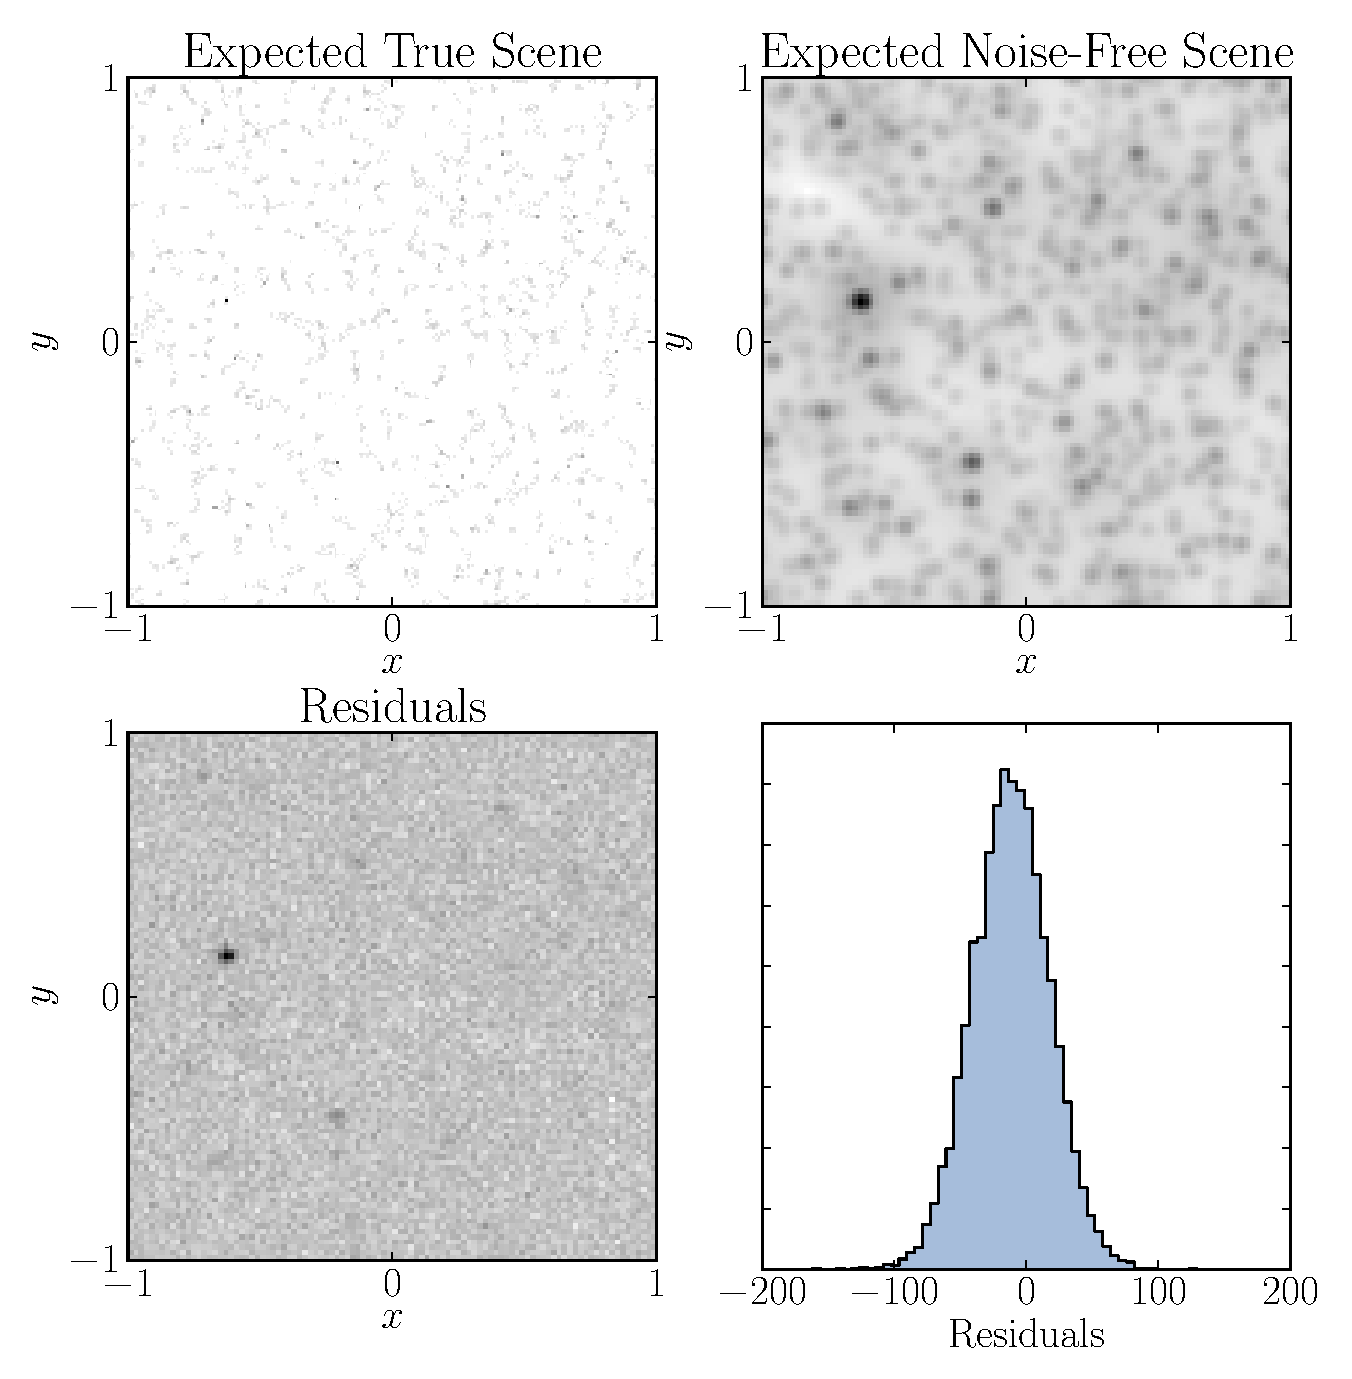
\includegraphics[width=\textwidth]{Figures/summaries.eps}
\end{center}
\caption{Summary images for test case 2. The upper left panel shows the posterior
mean high-resolution scene. The upper right panel shows the posterior mean scene
when observed at the resolution of the data, and the bottom panels show the
model residuals.
\label{fig:summaries}}
\end{figure}

As with test case 1, the PSF parameters $\{s_1, s_2, w\}$ and the noise parameters $\{\sigma_0, \eta\}$
were also inferred accurately with small uncertainties.

\section{Comparison to SExtractor}\label{sec:sex}
In the previous section we established that the inference of the catalogs from
the data is computationally feasible and that the number of stars and the
luminosity function can be inferred from the image data, albeit with moderate
uncertainty. We now compare this approach to an alternative analysis that makes
use of the standard
tool \sex. To achieve this, we executed \sex~on the two test images, for various
values of the detection threshold. This results in a set of catalogs
for each image, with more conservative thresholds resulting in less stars detected
as compared to more aggressive thresholds. The results for the number of stars in
the images are shown in Figure~\ref{fig:sex_N}. The main result is that
\sex~significantly underestimates the number of stars in the image for all
possible values of the detection threshold.

\begin{figure}[ht!]
\begin{center}
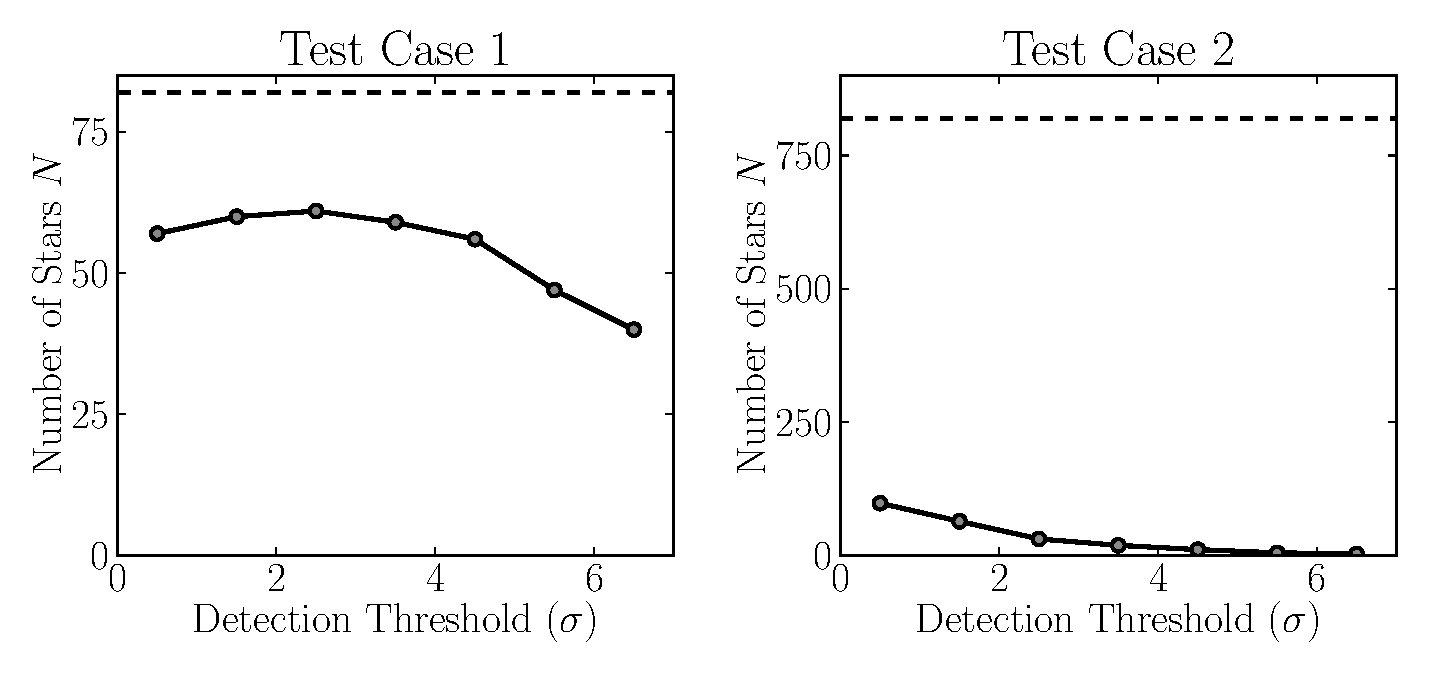
\includegraphics[width=\textwidth]{Figures/sex_N.eps}
\end{center}
\caption{The number of stars in the catalogs produced by \sex~compared with the
actual number of stars in the images. \sex~finds only a small fraction of the
stars actually present. This is to be expected in the high-$\sigma$ case as
\sex~then only searches for stars above a certain flux, but at the low-$\sigma$
end the number of stars is still drastically underestimated. Note that the true
numbers
of stars shown in these plots are $\sim$82\% of the values listed in
Figure~\ref{tab:truth} because here we only count those stars with positions
in $[-1, 1] \times [-1, 1]$.
\label{fig:sex_N}}
\end{figure}

For Test Case 2, we then took the catalog produced by \sex~for the $0.5\sigma$
threshold and fitted a broken power-law model to the list of fluxes in the catalog.
Such an approach might be used to study the luminosity function of a set of stars
in a field. The results of this inference are shown in Figure~\ref{fig:sex_inference}.
The inference spuriously rules out the true values of the parameters. This
occurs because the uncertainty in the stellar fluxes is not propagated through
to the inference of the luminosity function.

\begin{figure}[ht!]
\begin{center}
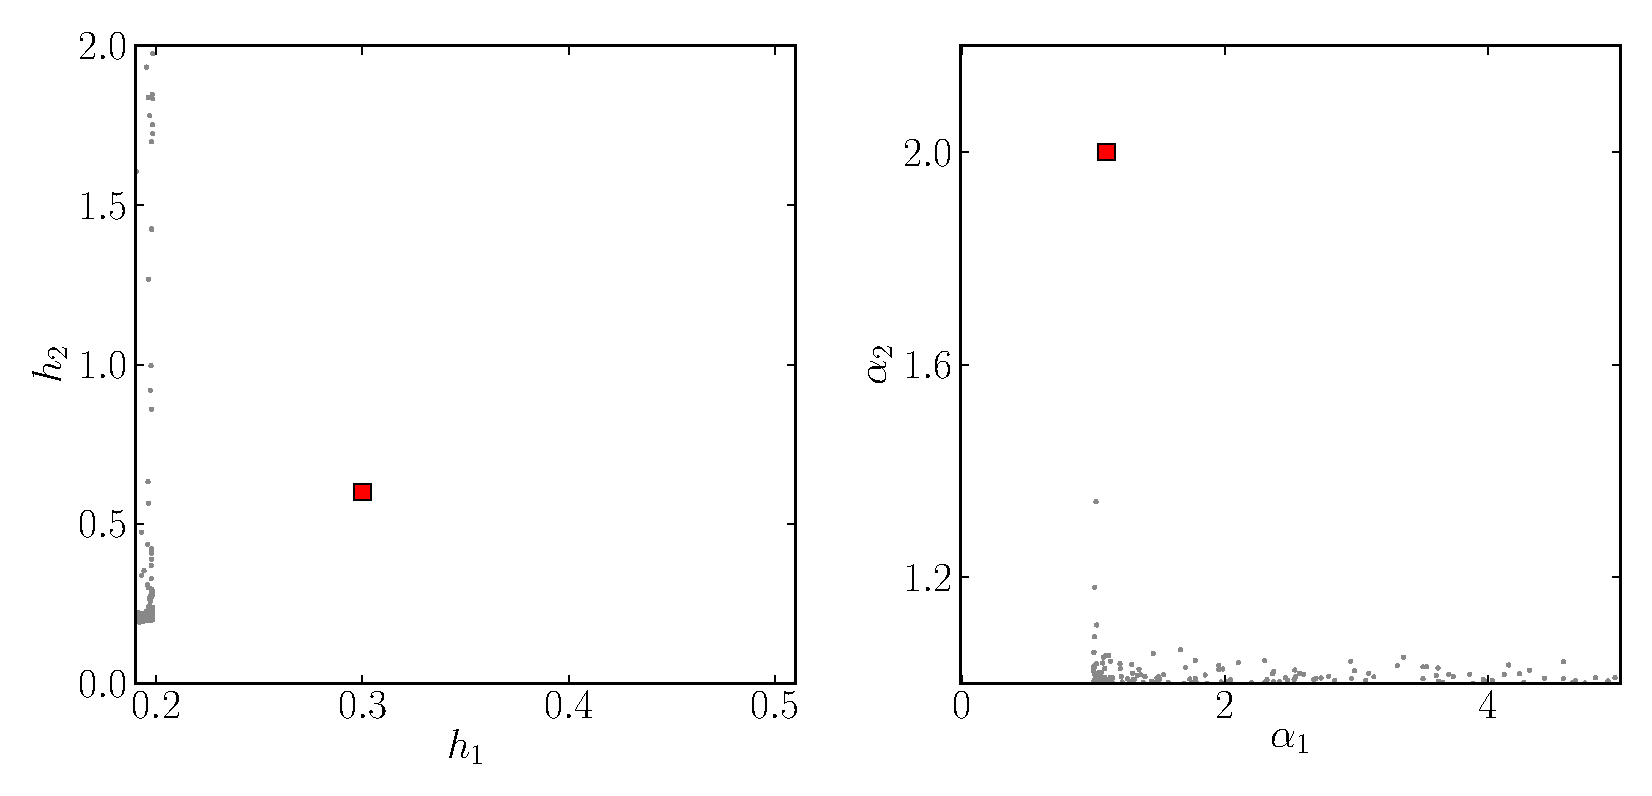
\includegraphics[width=\textwidth]{Figures/sex_inference.eps}
\end{center}
\caption{Inference of the luminosity function parameters using the $0.5\sigma$
catalog from \sex. Note that the inference appears to rule out regions around
the true input values. This occurs because the uncertainties in the existence
and fluxes of the faint stars are not taken into account. The true input values are plotted as filled squares.
\label{fig:sex_inference}}
\end{figure}

\section{Discussion and Conclusions}\label{sec:conclusion}
%What have we achieved?

In this paper we have developed and demonstrated a Bayesian approach to
making catalogs from astronomical images in the case where the image contains
only stars (or other point sources). The key idea is that instead of computing
a single catalog, the method creates a posterior probability distribution on
the space of possible catalogs that represents our state of knowledge about
the presence and properties of objects in the image. When this is done, the
uncertainties in the imaging are accurately propagated through to scientific
conclusions, for example about the luminosity function of the stars.
This approach was contrasted with a standard method of running \sex~and then
fitting a luminosity function to the fluxes in the catalog. This latter approach
was shown to produce incorrect inferences about the luminosity function.

We note that there are many limitations to the model presented in this paper.
In principle, our model should be a model of the physical state of the universe,
and not a simple model where the only stellar properties are a 2-D position and
a flux. Another limitation is that we have not considered multi-epoch or multi-band
imaging. In the former case, PSF variations and stellar motions may be relevant
\citep{lang}, and in the latter, a model for the spectral energy distributions
of the stars will need to be considered.

In practice, it may also be necessary to improve the model for the prior
distribution
of stellar positions and fluxes. One area where this is clearly needed is the
application of this approach to images of stellar clusters. The model would need
to be revised to take into account the fact that we expect the stars' positions
to be clustered together, whereas the current model implies a large prior
probability for the stars being scattered evenly across the image. In this and
other applications, the luminosity function would also require multiple
components, for example consisting of stars that are associated with a cluster
or a stream and those that are not.

Throughout this paper, we have also assumed that the pixel-convolved PSF can
be adequately modeled using simple components and that there are no PSF
variations across the field. Relaxing this assumption provides a significant
challenge for the future.

%What are the limitations of what we have done?  Limitations include
%PSF knowledge (and simplicity), simple number--flux relationship, no
%astrophysical model.  On the latter, I mean: No model of temperatures,
%masses, distances, reddening and so on.  We also haven't thought about
%multi-epoch, multi-band imaging, where you have to consider the
%motions and variations and spectral energy distributions of stars.  On
%this latter point, we should cite Lang et al (faint motion).  Each of
%these limitations should get its own paragraph, really.

%What kinds of new science will this enable?  One example would be IMF
%inference in dense stellar clusters.  Another could be modeling of
%distant galaxies in terms of their stellar components.  Most
%importantly, astrophysics can proceed without taking the hard,
%information-lossy step of fixing a catalog, somewhere between the raw
%data and the science of interest!

\section{Acknowledgements}
It is a pleasure to thank
  Jonathan Goodman (NYU),
  Fengji Hou (NYU),
  Dustin Lang (CMU),
  Geraint Lewis (Sydney), and
  Phil Marshall (Oxford)
for their comments and discussions.
The referee is thanked for their thoughtful comments which helped us to improve
the paper.
BJB would like to thank Tommaso Treu (UCSB) for his support, and
Wayne Stewart and Arden Miller (Auckland) for their encouragement and advice.
DFM and DWH were partially supported by
   the US National Science Foundation (grant IIS-1124794) and
   the US National Aeronautics and Space Administration (grant NNX12AI50G).

\appendix

\section{Broken Power-Law Distribution}\label{power_law}
The broken power-law distribution is based on a straightforward extension
to a simple power-law distribution (also known as a Pareto distribution,
particularly in the statistics literature). The power-law distribution for a
variable $x$ (given a lower cutoff $x=h$ and a slope $\alpha$) is defined by:
\begin{eqnarray}
p(x) &\propto&
\left\{
\begin{array}{lcl}
0, & & x < h \\
x^{-\alpha - 1} & & x \geq h.
\end{array}
\right.
\end{eqnarray}
In contrast, the broken power-law distribution for a variable $x$ is defined by
a lower cutoff $x=h_1$, two slopes $\{\alpha_1, \alpha_2\}$ and a break point
$x=h_2$:
\begin{eqnarray}
p(x) &\propto&
\left\{
\begin{array}{lcrl}
0, & & x < h_1 & \\
x^{-\alpha_1 - 1} & & h_1 \leq x \leq h_2 & \\
x^{-\alpha_2 - 1} & & x > h_2.
\end{array}
\right.
\end{eqnarray}
The free parameters of the broken power-law are:
\begin{eqnarray}
\beta = \{h_1, h_2, \alpha_1, \alpha_2\}.
\end{eqnarray}
With normalising terms included, the proportionality becomes an equality:
\begin{eqnarray}
p(x) &=&
\left\{
\begin{array}{lcr}
0, & & x < h_1 \\
Z_1^{-1}x^{-\alpha_1 - 1}, & & h_1 \leq x \leq h_2 \\
Z_2^{-1}x^{-\alpha_2 - 1}, & & x > h_2.
\end{array}
\right.
\end{eqnarray}
Two conditions will be used to determine the normalizers $Z_1$ and $Z_2$.
Firstly, the probability density function (PDF) should be continuous at $x=h_2$:
\begin{eqnarray}
Z_1^{-1}h_2^{-\alpha_1 - 1} &=& Z_2^{-1}h_2^{-\alpha_2 - 1}\\
\implies
Z_2 &=& Z_1h_2^{\alpha_1-\alpha_2}
\end{eqnarray}
The second condition is that the total probability must be 1:
\begin{eqnarray}
\int_{h_1}^{h_2} Z_1^{-1} x^{-\alpha_1 - 1} \, dx
+
\int_{h_2}^\infty Z_2^{-1} x^{-\alpha_2 - 1} \, dx
&=& 1 \\
Z_1^{-1}\alpha_1^{-1}\left[h_1^{-\alpha_1} - h_2^{-\alpha_1}\right]
+
Z_2^{-1}\alpha_2^{-1}h_2^{-\alpha_2}
&=& 1 \\
Z_1^{-1}\alpha_1^{-1}\left[h_1^{-\alpha_1} - h_2^{-\alpha_1}\right]
+
Z_1^{-1}h_2^{\alpha_2-\alpha_1}\alpha_2^{-1}h_2^{-\alpha_2}
&=& 1
\end{eqnarray}
\begin{eqnarray}
\implies
Z_1 &=& \alpha_1^{-1}\left[h_1^{-\alpha_1} - h_2^{-\alpha_1}\right]
+
h_2^{-\alpha_1}\alpha_2^{-1}.
\end{eqnarray}
The cumulative distribution (CDF) is a useful property of a probability
distribution and is given by the antiderivative of the PDF:
\begin{eqnarray}
P(X \leq x) = F(x) &=&
\left\{
\begin{array}{lcr}
0, & & x < h_1 \\
(Z_1\alpha_1)^{-1}\left(h_1^{-\alpha_1} - x^{-\alpha_1}\right), & & h_1 \leq x \leq h_2 \\
1 - (Z_2\alpha_2)^{-1}x^{-\alpha_2}, & & x > h_2.
\end{array}
\right.
\end{eqnarray}
The inverse of the CDF is also useful and is given by:
\begin{eqnarray}
F^{-1}(u) &=&
\left\{
\begin{array}{lcr}
\left[h_1^{-\alpha_1} - uZ_1\alpha_1\right]^{-1/\alpha_1}, & & 0 < u < 1 - (Z_2\alpha_2)^{-1}h_2^{-\alpha_2}\\
\left[Z_2\alpha_2(1-u)\right]^{-1/\alpha_2},& & 1 - (Z_2\alpha_2)^{-1}h_2^{-\alpha_2}< u < 1.
\end{array}
\right.
\end{eqnarray}
An example of a broken power-law distribution is shown in Figure~\ref{fig:powerlaw}.
\begin{figure}[ht!]
\begin{center}
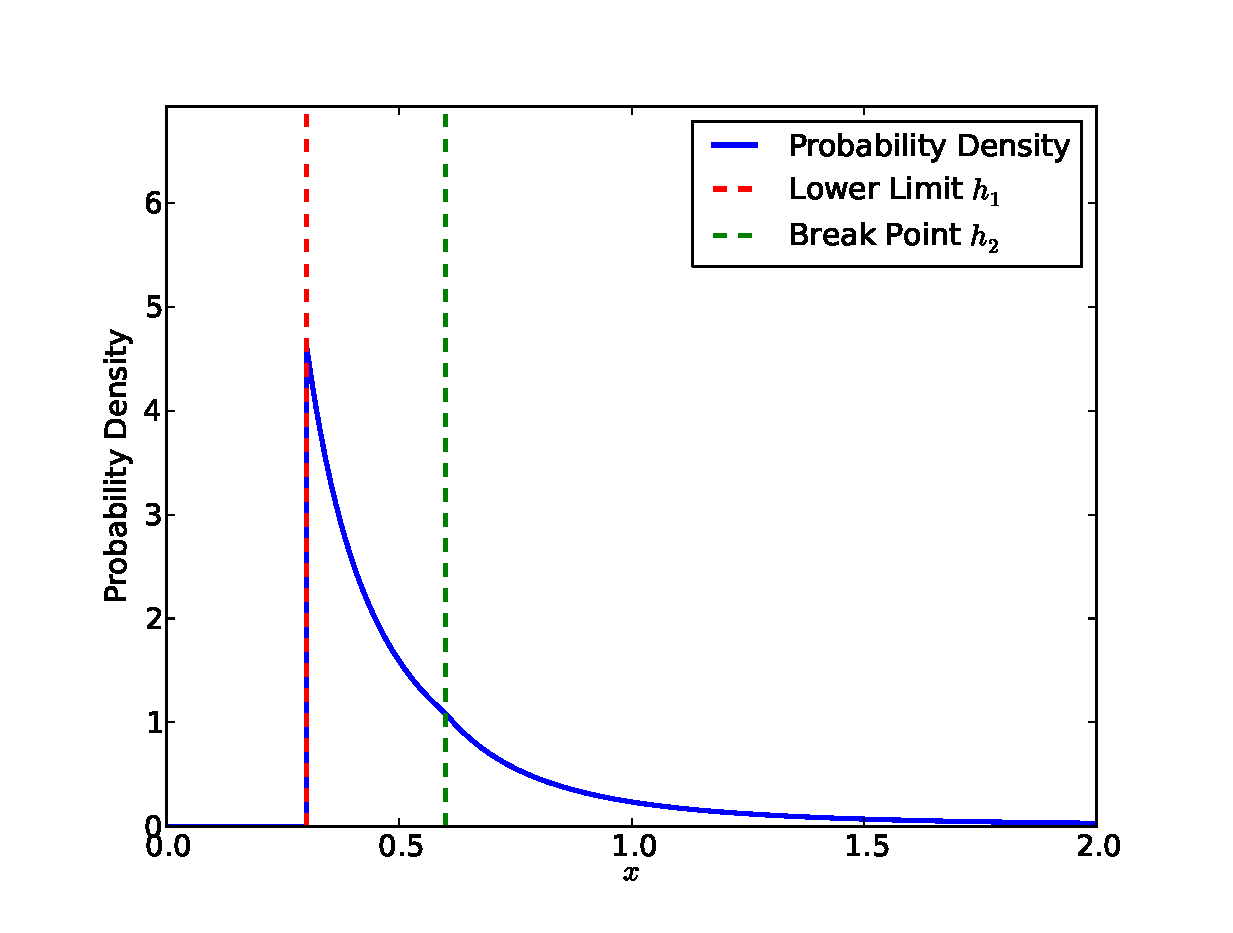
\includegraphics[width=\textwidth]{Figures/broken.eps}
\caption{A broken power-law distribution. The parameter values for this
particular PDF were
$\{h_1, h_2, \alpha_1, \alpha_2\} = \{0.3, 0.6, 1.1, 2\}$, i.e. the same
parameter values used to make the simulated data.
\label{fig:powerlaw}}
\end{center}
\end{figure}



\section{Proposal Distributions}
To implement Metropolis-Hastings moves for the space of possible catalogs,
proposal distributions are required. See Table~\ref{tab:proposals} for a list of
proposal distributions used in this study.

\begin{table}\footnotesize
\begin{center}
\begin{tabular}{|c|c|c|}
\hline
Parameter & Proposal & Notes\\
\hline
$N$ & $N \to N + \delta_N$ & Generate $\delta_N$ new stars from
$p(x, y, f|\beta)$.\\
$N$ & $N \to N - \delta_N$ & Remove $\delta_N$ stars, chosen at random\\
$\beta$ & $\beta \to \beta + \delta_\beta$ & Transform
stars' fluxes correspondingly\\
$\beta$ & $\beta \to \beta + \delta_\beta$ & Fix stars' fluxes, put extra
term in acceptance probability \\
$(x_i,y_i)$ & $(x_i,y_i) \to (x_i,y_i)+(\delta_x, \delta_y)$ & Can move $>1$ star
in a single step \\
$f$ & $f \to f + \delta_f$ & Can move $>1$ stars' fluxes in a single step\\
\hline
\end{tabular}
\end{center}
\caption{All $\delta$ parameters are drawn from multi-scale distibutions such
that the largest steps are of order the prior width, and the smallest steps
are of order $10^{-6}$ times the prior width.\label{tab:proposals}}
\end{table}






%\subsection{Future Possibilities}
%{\bf Hogg}: {\it I think this problem is important enough and general enough
%that we should spend some time working on some ideas there.  If we can sample
%over image explanations, our powers in astronomy will be awesome
%beyond our wildest imaginings.}

%\subsection{Genetic Moves}
%Here I will sketch some ideas...




\begin{thebibliography}{99}
\bibitem[Bertin and
Arnouts(1996)]{sextractor} Bertin, E., Arnouts, S.\ 1996.\ SExtractor: Software for source extraction.\ Astronomy and Astrophysics Supplement Series 117, 393-404.

\bibitem[\protect\citeauthoryear{Brewer, P{\'a}rtay,
\& Cs{\'a}nyi}{2011}]{dnest} Brewer B.~J., P{\'a}rtay L.~B.,
Cs{\'a}nyi G., 2011, Statistics and Computing, 21, 4, 649-656. arXiv:0912.2380

\bibitem[Brewer et al.(2011)]{2011MNRAS.412.2521B} Brewer, B.~J., Lewis,
G.~F., Belokurov, V., Irwin, M.~J., Bridges, T.~J., Evans, N.~W.\ 2011.\
Modelling of the complex CASSOWARY/SLUGS gravitational lenses.\ Monthly
Notices of the Royal Astronomical Society 412, 2521-2529

\bibitem[Caticha(2009)]{caticha} Caticha, A.\ 2009.\
Quantifying Rational Belief.\ American Institute of Physics Conference
Series 1193, 60-68.

\bibitem[Cox(1946)]{cox} Cox, R.~T., 1946, Probability, Frequency, and Reasonable Expectation. 1946. American Journal of Physics 14 14, 1-13.

\bibitem[Feroz et al.(2011)]{2011MNRAS.415.3462F} Feroz, F., Balan, S.~T.,
Hobson, M.~P.\ 2011.\ Detecting extrasolar planets from stellar radial
velocities using Bayesian evidence.\ Monthly Notices of the Royal
Astronomical Society 415, 3462-3472.

\bibitem[\protect\citeauthoryear{Feroz, Hobson,
\& Bridges}{2009}]{multinest} Feroz F., Hobson M.~P., Bridges M., 2009, MNRAS, 398, 1601

\bibitem[Foreman-Mackey et al.(2012)]{emcee} Foreman-Mackey, 
D., Hogg, D.~W., Lang, D., \& Goodman, J.\ 2012, emcee: The MCMC Hammer, arXiv:1202.3665 

\bibitem[\protect\citeauthoryear{Goodman \& Weare}{2010}]{goodman}
Goodman, J., Weare, J., 2010, Ensemble Samplers with Affine Invariance, Comm. App. Math. Comp. Sci., 5, 6.

\bibitem[\protect\citeauthoryear{Green}{1995}]{rjmcmc}
Green, P.~J., 1995, Reversible Jump Markov Chain Monte Carlo Computation and Bayesian Model Determination, Biometrika 82 (4): 711–732.

\bibitem[Harkness and Green(2000)]{object} Harkness, M.~A. and Green, P.~J., 2000,
Parallel chains, delayed rejection and reversible jump MCMC for object recognition,
British Machine Vision Conference Proceedings.

\bibitem[Hobson 
\& McLachlan(2003)]{2003MNRAS.338..765H} Hobson, M.~P., \& McLachlan, C.\ 2003, \mnras, 338, 765 

\bibitem[Hogg(2012)]{hogg} Hogg, D.~W.\ 2012.\ Data analysis
recipes: Probability calculus for inference.\ ArXiv e-prints
arXiv:1205.4446.

\bibitem[Hogg and Lang(2011)]{2011EAS....45..351H} Hogg, D.~W., Lang, D.\
2011.\ Telescopes don't make catalogues!.\ EAS Publications Series 45,
351-358.

\bibitem[Irwin(1985)]{irwin} Irwin, M.~J.\ 1985, \mnras, 214,
575

\bibitem[Jasra et al(2005)]{label_switching} Jasra, A., Holmes, C.~C, and
Stephens, D.~A., Markov Chain Monte Carlo Methods and the Label Switching
Problem in Bayesian Mixture Modeling, Statistical Science
Vol. 20, No. 1, pp. 50-67

\bibitem[Jaynes(2003)]{jaynes} Jaynes, E.~T., 2003, Probability Theory: The
Logic of Science, ISBN 0521592712, Cambridge University Press, June 2003.

\bibitem[Kelly et al.(2008)]{2008ApJ...682..874K} Kelly, B.~C., Fan, X.,
\& Vestergaard, M.\ 2008, ApJ, 682, 874

\bibitem[Kirkpatrick et al.(1983)]{annealing}
Kirkpatrick, S., Gelatt, C.~D., Vecchi, M.~P., 1983,
Optimization by Simulated Annealing, Science 220 (4598): 671–680.

\bibitem[Lang et al.(2009)]{lang} Lang, D., Hogg, D.~W., 
Jester, S., \& Rix, H.-W.\ 2009, \aj, 137, 4400 

\bibitem[Lupton et al.(2001)]{photo}
Lupton,~R., Gunn,~J.~E., Ivezic,~Z., Knapp,~G.~R., Kent,~S.~M., \& Yasuda,~N., 2001, ASPC, 238, 269

\bibitem[Mackay(2003)]{mackay} Mackay, D.~J.~C., 2003, Information Theory,
Inference and Learning Algorithms, Cambridge University Press, UK.

\bibitem[Magain et 
al.(2007)]{2007A&A...461..373M} Magain, P., Courbin, F., Gillon, M., et al.\ 2007, \aap, 461, 373 

\bibitem[Metchev 
\& Grindlay(2002)]{2002MNRAS.335...73M} Metchev, S.~A., \& Grindlay, J.~E.\ 2002, \mnras, 335, 73 

\bibitem[Neal(2001)]{neal} Neal, R.~M., 2001, 
Annealed importance sampling, Statistics and Computing, vol. 11, pp. 125-139.

\bibitem[\protect\citeauthoryear{Skilling}{1998}]{massinf}
Skilling J., 1998, Massive Inference and Maximum Entropy, in Maximum Entropy
and Bayesian Methods, Kluwer Academic Publishers, Dordrecht/Boston/London p.14

\bibitem[\protect\citeauthoryear{Skilling}{2006}]{skilling} Skilling, J., 2006, Nested Sampling for General Bayesian Computation, Bayesian Analysis 4, pp. 833-860.

\bibitem[Stetson(1987)]{1987PASP...99..191S} Stetson, P.~B.\ 1987, \pasp,
99, 191

\bibitem[Zhang et al.(2009)]{2009PASP..121.1429Z} Zhang, Z.~W., Kim, D.~W., 
Wang, J.~H., et al.\ 2009, \pasp, 121, 1429 
\end{thebibliography}

\end{document}

